\section{Recurrent Neural Networks \label{ssec: RNNs}}
    Consider the following sentences as inputs to a \gls{nn}:

    \begin{table}[H]
    \begin{tabular}{|l|l|l|l|l|l|}
        \hline
        $i$   & 0   & 1   & 2     & 3    & 4    \\ \hline
        $s_1$ & The & sky & isn't & blue &      \\ \hline
        $s_2$ & The & sky & is    & blue &      \\ \hline
        $s_3$ & The & sky & is    & not  & blue \\ \hline
    \end{tabular}
    \centering
    \end{table}
    \noindent %Using word \glspl{embedding} (a map from words to vectors that represent the word's meaning, formally introduced in Sec. \ref{ssec: word embeddings}) we are able to turn these words into meaningful numbers that the \gls{nn} can process, but due to the (lack of) structure within sentences, we face another issue:
    Sentences $s_1$ and $s_2$ have different meanings, but because most words are the same, the inputs would appear relatively similar a hypothetical \gls{model} and yield similar outputs $\hat{Y}$. $s_1$ and $s_3$ have the same meaning, but are of different length. Therefore, in our hypothetical \gls{nn}, the inputs in positions $i = \{2, 3, 4\}$ are different, leading to potentially quite different outputs $\hat{Y}$.

    The problem is that in language, the absolute position of words within sentences is not particularly important, but relative positions and context-words are: One word,``not", can change the meaning of the entire sentence dramatically.

     \Glspl{rnn} address these concerns and can process sequences of variable length such as sentences. \Glspl{rnn} use \glspl{neuron} as computational units in the same way traditional \glspl{nn} do, but instead of simply connecting \glspl{neuron} from the previous layer to \glspl{neuron} of the next layer, they connect \glspl{neuron} \textit{within} a single layer, so that they form a directed graph. Every \gls{neuron} $n_i$ then corresponds to one input in the sequence (e.g. one word in a sentence) and calculations are performed in a temporal direction: a hidden state of numbers is created at $n_1$, and repeatedly passed on to the next \gls{neuron} $n_{i+1}$, changed in a way determined by the $i+1$th input and the \gls{neuron}'s parameters $\theta$ and passed on again. At the last \gls{neuron}, every input has impacted the hidden state in some sensible way (specified by $\theta$) and the information can be passed to the next layer for further processing. A short example is given in Fig. \ref{fig:rnn}.
     
     \begin{figure}[ht]
        \centering
        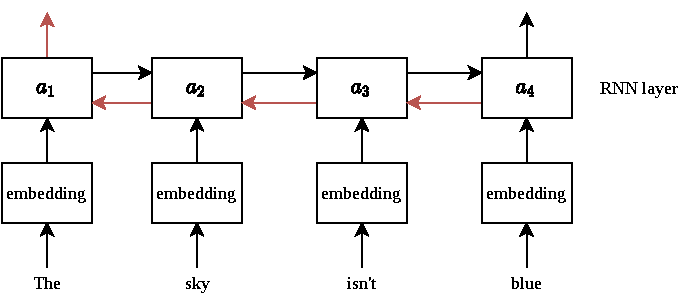
\includegraphics{rnn.pdf}
        \caption{The \gls{rnn} layer is given an input sequence of word \glspl{embedding}, calculates a hidden state depending on the first \gls{embedding} and the weights of the first neuron, and passes this hidden state on to the next \gls{neuron} within the \gls{rnn} layer. 
        %Every \gls{neuron} modifies the hidden state based on its weights and the input \gls{embedding} at its position and passes the modified state on. At the end of the sentence, the hidden state is passed on as the output of the layer. 
        In a bidirectional \gls{model} (red arrows), a second hidden state is passed through the layer ``backwards".}
        \label{fig:rnn}
    \end{figure}


    \subsection{\gls{rnn} Architectures \label{ssec: rnn architectures}}
    The exact calculations that combine the hidden state with new inputs and parameters are determined by the internal architecture of the \glspl{neuron}. The most prominently used architectures (which we also use in our \gls{da} classification \gls{model}) are \gls{lstm}\cite{hochreiter1997long} and \gls{gru}\cite{chung2014empirical} architectures, both of which are capable of attaining state of the art performance on \gls{nlp} tasks\cite{huang2015bidirectional}.
    %%%%%%%%%%%%%%%%%%%

    \subsection{Bi-directional RNNs \label{ssec: bidirectional RNN}}
    If an \gls{rnn} layer is bi-directional, in addition to the hidden state being passed through the layer in a forward direction ($n_i \rightarrow n_{i+1}$), another hidden state is passed through the layer backwards ($n_{i-1} \leftarrow n_i$). This improves performance in many \gls{nlp} tasks, because e.g.  the impact of a given word on the meaning of a sentence does not only depend on its preceding, but also on its succeeding words\cite{schuster1997bidirectional}. This means the \gls{rnn} layer has two outputs, one for the forwards pass and one for the backwards pass. This is indicated in red in Fig. \ref{fig:rnn}.

    \subsection{Outputting Hidden States \label{ssec: outputting hidden states}}
    In some cases, it is useful for the \gls{rnn} to have one output for every element in the sequence, not just one output at the end of the sequence. The different elements of the sequence still impact eachother's output, but now the output is a sequence of length equal to the input sequence. In that case, the hidden states of every \gls{neuron} are simply output to the next layer\cite{mlTextbook}.

    %\subsubsection{When to Output Hidden States?}
    %Consider for example the following two different \glspl{model}, each with a different goal, but both taking a sequence of words $\mathcal{S}$ as an input.

    %The first \gls{model},
    %\begin{equation}
    %    \hat{f}_{\text{pos}}: \mathcal{S} \rightarrow \mathcal{P},
    %\end{equation}
    %outputs a sequence of \gls{pos} tags $\mathcal{P}$, one for every word e.g.
    %    \begin{equation*}
    %    \text{[The, house, is, green] $\rightarrow$ [article, %noun, verb, adjective]}.
    %    \end{equation*}
    %We still want the words to affect eachother's tags (i.e. green could be an adjective or a noun, depending on the other words in the sentence), but we want one tag for every word in the sequence. We want to map $N$ words $ \rightarrow N$ tags. In this case we want to return the $N$ hidden states as outputs.

    %The second \gls{model},
    %\begin{equation}
    %    \hat{f}_{q\Bar{q}}: \mathcal{S} \rightarrow q,
    %\end{equation}
    %outputs whether or not the sequence of words was a question or not, $q$. E.g.
    %    \begin{align*}
    %    \text{[The, house, is, green]} &\rightarrow \text{not a %question}\\
    %    \text{[Is, the, house, green]} &\rightarrow \text{question}.
    %    \end{align*}
    %It maps $N$ words $\rightarrow 1$ tag. In this case we want to output only one value, encapsulating the entire sequence; only the last \gls{neuron}'s value is returned.
    When we are mapping a sequence of length $N$ to a single tag (many to one) we only return the hidden state of the final \gls{neuron} encapsulating the entire sequence. When we instead map a sequence of length $N$ to an output sequence of tags of length $N$ instead, we return all hidden states.
